\documentclass[11pt]{article}

\usepackage{amsmath}
\usepackage{amsfonts} 
\usepackage{amsthm}
\usepackage{blkarray}
\usepackage{caption}
\usepackage{enumitem} 
\usepackage{mathtools}
\usepackage[table]{xcolor}
\usepackage{tikz}
\usepackage{import}
\usepackage[top=2cm,bottom=2cm,left=1.75cm,right=2cm,marginparwidth=1.75cm]{geometry}
\setlength{\parindent}{0cm}
\newcommand{\R}{\mathbb{R}}
\newcommand{\sm}{\scriptsize}
\newcommand{\F}{\mathcal{F}}
\newcommand\itm[1]{\item[\textbf{#1}]}
\newcommand{\incid}{{-}\!{\bullet}\!{-}}
\newcommand{\n}{\vspace{0.3cm}}
\newcommand\cl{\cellcolor{blue!20}}

\usetikzlibrary{decorations.pathreplacing,decorations.markings}
\tikzset{
  % style to apply some styles to each segment of a path
  on each segment/.style={
    decorate,
    decoration={
      show path construction,
      moveto code={},
      lineto code={
        \path [#1]
        (\tikzinputsegmentfirst) -- (\tikzinputsegmentlast);
      },
      curveto code={
        \path [#1] (\tikzinputsegmentfirst)
        .. controls
        (\tikzinputsegmentsupporta) and (\tikzinputsegmentsupportb)
        ..
        (\tikzinputsegmentlast);
      },
      closepath code={
        \path [#1]
        (\tikzinputsegmentfirst) -- (\tikzinputsegmentlast);
      },
    },
  },
  % style to add an arrow in the middle of a path
  mid arrow/.style={postaction={decorate,decoration={
        markings,
        mark=at position .5 with {\arrow[#1]{stealth}}
      }}},
}

\def\lc{\left\lceil}   
\def\rc{\right\rceil}
\def\lf{\left\lfloor}   
\def\rf{\right\rfloor}

\newtheorem{theorem}{Theorem}

\title{\vspace{-1.5cm}MATH 5707 Homework 4}
\author{Fletcher Gornick}
\date{March 27, 2023}

\begin{document}
\maketitle
\begin{itemize}
  \itm{11.1.1} For each of the following networks, determine all possible flows and the value of a maximum flow. \n\\
  \resizebox{!}{6.5cm}{
    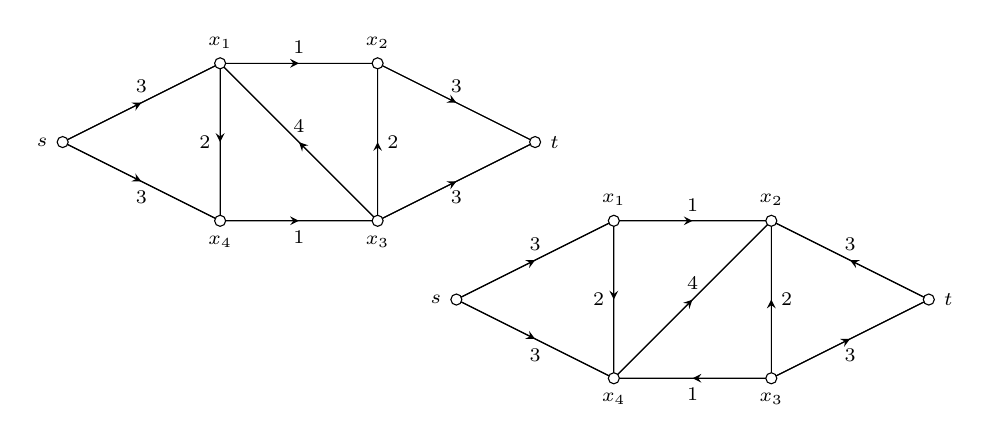
\begin{tikzpicture}
      \tikzset{
        dot/.style = {circle, draw, fill=white, minimum size=#1, inner sep=0pt, outer sep=0pt},
        dot/.default = 4pt
      }
      \node[dot,label=left:{\sm \(s\)}] (sa) at (0,3) {};
      \node[dot,label=right:{\sm \(t\)}] (ta) at (6,3) {};

      \node[dot,label=above:{\sm \(x_1\)}] (x1a) at (2,4) {};
      \node[dot,label=above:{\sm \(x_2\)}] (x2a) at (4,4) {};
      \node[dot,label=below:{\sm \(x_3\)}] (x3a) at (4,2) {};
      \node[dot,label=below:{\sm \(x_4\)}] (x4a) at (2,2) {};

      \node[dot,label={left:\sm \(s\)}] (sb) at (5,1) {};
      \node[dot,label={right:\sm \(t\)}] (tb) at (11,1) {};


      \node[dot,label=above:{\sm \(x_1\)}] (x1b) at (7,2) {};
      \node[dot,label=above:{\sm \(x_2\)}] (x2b) at (9,2) {};
      \node[dot,label=below:{\sm \(x_3\)}] (x3b) at (9,0) {};
      \node[dot,label=below:{\sm \(x_4\)}] (x4b) at (7,0) {};

      \path [draw=black, postaction={on each segment={mid arrow=black}}]
        (sa) edge node[above] {\sm 3} (x1a)
        (sa) -- (x1a)

        (sa) edge node[below] {\sm 3} (x4a)
        (sa) -- (x4a)

        (x1a) edge node[above] {\sm 1} (x2a)
        (x1a) -- (x2a)

        (x2a) edge node[above] {\sm 3} (ta)
        (x2a) -- (ta)

        (x4a) edge node[below] {\sm 1} (x3a)
        (x4a) -- (x3a)

        (x3a) edge node[below] {\sm 3} (ta)
        (x3a) -- (ta)

        (x1a) edge node[left] {\sm 2} (x4a)
        (x1a) -- (x4a)

        (x3a) edge node[right] {\sm 2} (x2a)
        (x3a) -- (x2a)

        (x3a) edge node[above] {\sm 4} (x1a)
        (x3a) -- (x1a)
      ;

      \path [draw=black, postaction={on each segment={mid arrow=black}}]
        (sb) edge node[above] {\sm 3} (x1b)
        (sb) -- (x1b)

        (sb) edge node[below] {\sm 3} (x4b)
        (sb) -- (x4b)

        (x1b) edge node[above] {\sm 1} (x2b)
        (x1b) -- (x2b)

        (tb) edge node[above] {\sm 3} (x2b)
        (tb) -- (x2b)

        (x3b) edge node[below] {\sm 1} (x4b)
        (x3b) -- (x4b)

        (x3b) edge node[below] {\sm 3} (tb)
        (x3b) -- (tb)

        (x1b) edge node[left] {\sm 2} (x4b)
        (x1b) -- (x4b)

        (x3b) edge node[right] {\sm 2} (x2b)
        (x3b) -- (x2b)

        (x4b) edge node[above] {\sm 4} (x2b)
        (x4b) -- (x2b)
      ;
    \end{tikzpicture}
  } \n

  For the first graph, we have the following possible flows (2 being the maximum): \n\\
  \import{./}{11.1.1.tex}

    For the second graph, since \(x_3\) has no inward capacity in, and it's the only vertex that moves out to \(t\), the only possible flow is the zero-flow. \n


  \itm{11.2.1} In the following network:
  \begin{center}
    \resizebox{!}{4cm}{
      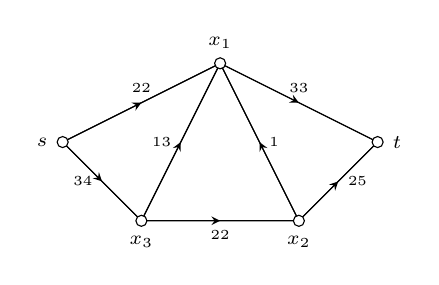
\begin{tikzpicture}
        \tikzset{
          dot/.style = {circle, draw, fill=white, minimum size=#1, inner sep=0pt, outer sep=0pt},
          dot/.default = 4pt
        }
        \node[dot,label=left:{\sm \(s\)}] (s) at (0,1) {};
        \node[dot,label=right:{\sm \(t\)}] (t) at (4,1) {};

        \node[dot,label=above:{\sm \(x_1\)}] (x1) at (2,2) {};
        \node[dot,label=below:{\sm \(x_2\)}] (x2) at (3,0) {};
        \node[dot,label=below:{\sm \(x_3\)}] (x3) at (1,0) {};


        \path [draw=black, postaction={on each segment={mid arrow=black}}]
          (s) edge node[above] {\tiny 22} (x1)
          (s) -- (x1)

          (x1) edge node[above] {\tiny 33} (t)
          (x1) -- (t)

          (s) edge node[left] {\tiny 34} (x3)
          (s) -- (x3)

          (x3) edge node[below] {\tiny 22} (x2)
          (x3) -- (x2)

          (x2) edge node[right] {\tiny 25} (t)
          (x2) -- (t)

          (x3) edge node[left] {\tiny 13} (x1)
          (x3) -- (x1)

          (x2) edge node[right] {\tiny 1} (x1)
          (x2) -- (x1)

        ;
      \end{tikzpicture}
    }
  \end{center}
  \begin{enumerate}[label=(\alph*)]
      \item determine all cuts; \n\\
        \(K_1 = \left(\{s\}, \{x_1,x_2,x_3,t\}\right)\), capacity \(c(K_1) = 22 + 34 = 56\) \\
        \(K_2 = \left(\{s,x_1\}, \{x_2,x_3,t\}\right)\), capacity \(c(K_2) = 34 + 33 = 67\) \\
        \(K_3 = \left(\{s,x_2\}, \{x_1,x_3,t\}\right)\), capacity \(c(K_3) = 22 + 34 + 1 + 25 = 82\) \\
        \(K_4 = \left(\{s,x_3\}, \{x_1,x_2,t\}\right)\), capacity \(c(K_4) = 22 + 13 + 22 = 57\) \\
        \(K_5 = \left(\{s,x_1,x_2\}, \{x_3,t\}\right)\), capacity \(c(K_5) = 34 + 33 + 25 = 92\) \\
        \(K_6 = \left(\{s,x_1,x_3\}, \{x_2,t\}\right)\), capacity \(c(K_6) = 22 + 33 = 55\) \\
        \(K_7 = \left(\{s,x_2,x_3\}, \{x_1,t\}\right)\), capacity \(c(K_7) = 22 + 13 + 1 + 25 = 81\) \\
        \(K_8 = \left(\{s,x_1,x_2,x_3\}, \{t\}\right)\), capacity \(c(K_8) = 33 + 25 = 58\) \n

      \item find the capacity of a minimum cut; \n\\
        Cut \(K_6\) yields capacity 55. \n

      \item show that the flow indicated is a maximum flow. \n\\
        \(x_1\) and \(x_2\) are the only vertices connected to \(t\).  \(x_1\) can have a maximum of 33 flow out, and \(x_2\) can have a maximum of 22 flow in, so our max flow can't be more than 55, here's what this flow looks like:

      \begin{center}
        \resizebox{!}{4cm}{
          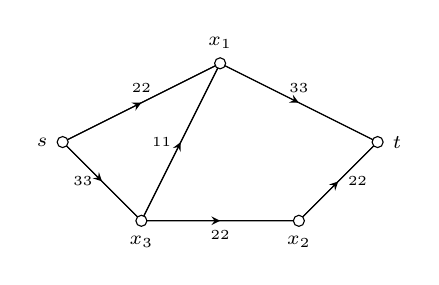
\begin{tikzpicture}
            \tikzset{
              dot/.style = {circle, draw, fill=white, minimum size=#1, inner sep=0pt, outer sep=0pt},
              dot/.default = 4pt
            }
            \node[dot,label=left:{\sm \(s\)}] (s) at (0,1) {};
            \node[dot,label=right:{\sm \(t\)}] (t) at (4,1) {};

            \node[dot,label=above:{\sm \(x_1\)}] (x1) at (2,2) {};
            \node[dot,label=below:{\sm \(x_2\)}] (x2) at (3,0) {};
            \node[dot,label=below:{\sm \(x_3\)}] (x3) at (1,0) {};


            \path [draw=black, postaction={on each segment={mid arrow=black}}]
              (s) edge node[above] {\tiny 22} (x1)
              (s) -- (x1)

              (x1) edge node[above] {\tiny 33} (t)
              (x1) -- (t)

              (s) edge node[left] {\tiny 33} (x3)
              (s) -- (x3)

              (x3) edge node[below] {\tiny 22} (x2)
              (x3) -- (x2)

              (x2) edge node[right] {\tiny 22} (t)
              (x2) -- (t)

              (x3) edge node[left] {\tiny 11} (x1)
              (x3) -- (x1)
            ;
          \end{tikzpicture}
        }
      \end{center}
    \end{enumerate} \n



  \itm{11.2.2} Show that, if there exists no directed \((x, y)\)-path in \(N\), then the value of a maximum flow and the capacity of a minimum cut are both zero.
  \begin{proof}
    Since \(f \colon A \to \R_{\geq 0}\), we know that the flow is always at least 0, and by theorem 11.1, we know \(\text{val}(f) \leq c(K)\) for any cut \(K\).  So if we can show that (given there exists no \((x,y)\)-path in \(N\)) the capacity of a minimum cut on \(N\) is zero, then it logically follows that the max flow is also zero. \n

    Now, suppose to the contrary, the minimum cut has capacity \(\geq 1\), we will attempt to construct a directed \((x,y)\)-path in \(N\). \n

  First, take the cut \(\left(S_1, \overline{S_1}\right)\) where \(S_1 = \{x\}\), and \(S_i := N \setminus S_i\) for each \(i\).  Since our minimum cut has nonzero capacity, there exists edge \(v_1 \in \overline{S_1}\) such that \(c(xv_1) \geq 1\).  If \(v_1 = y\), then we've reached a contradiction, so assume not.  Now construct set \(S_2 = S_1 \cup \{v_1\}\).  Before proceeding, note that there's clearly a directed \((x,v_1)\)-path in \(N\), this path just consists of the edge \(xv_1\). \n

  Now take an arbitrary step \(i\) in this process, and assume each vertex \(v \in S_i\) is reachable by \(x\) (base case covered in previous paragraph).  We know our cut \(\left(S_i, \overline{S_i}\right)\) has positive cut capacity, meaning there's a \(u \in S_i\) with a directed edge \(e \in A(N)\) to some \(v \in \overline{S_i}\).  Now we can just take the directed path from \(x\) to \(u \in S_i\), and add on our edge \(e\), giving us new cut \(\left(S_{i+1}, \overline{S_{i+1}}\right)\), where all vertices in \(S_{i+1}\) are reachable via a directed path from \(x\). \n

  Assuming our network contains a finite number of vertices, there will inevitably come a point where we have some \(u \in S_j\) with a directed edge to \(y \in \overline{S_j}\), meaning we've found a directed \((x,y)\)-path in \(N\), which is a contradiction.  Therefore, if there exists no \((x,y)\)-path in \(N\), we can conclude that the minimum cut and the maximum flow are both zero.
  \end{proof} \n
  


  \itm{11.2.3} If \(\left(S, \overline{S}\right)\) and \(\left(T, \overline{T}\right)\) are minimum cuts in \(N\), show that \(\left(S \cap T, \overline{S \cap T}\right)\) and \(\left(S \cup T, \overline{S \cup T}\right)\) are also minimum cuts in \(N\).
  \begin{proof}
    From 11.3, we know the value of the maximum flow of any network is equal to the capacity of it's minimum cut.  This means that for max flow \(f\), each edge across our minimum cut is \(f\)-saturated, and each edge going back is \(f\)-zero.  So if we can show this is the case for our two cuts \(\left(S \cap T, \overline{S \cap T}\right)\) and \(\left(S \cup T, \overline{S \cup T}\right)\), then we can conclude they are minimum cuts. \n

    For any sets \(X,Y\), \(\overline{X \cap Y} = \overline{X} \cup \overline{Y}\), and \(\overline{X \cup Y} = \overline{X} \cap \overline{Y}\) by De Morgan's laws.  So we can rewrite our two cuts as \(\left(S \cap T, \overline{S} \cup \overline{T}\right)\) and \(\left(S \cup T, \overline{S} \cap \overline{T}\right)\) \n

    First, for cut \(\left(S \cap T, \overline{S} \cup \overline{T}\right)\), we know every forward edge is \(f\)-saturated because if \(a \in \left(S \cap T, \overline{S} \cup \overline{T}\right)\), then it has it's tail in \(S\) as well as \(T\), it must also have it's head in either \(\overline{S}\) or \(\overline{T}\).  If \(a\) has head in \(\overline{S}\), then \(a \in (S, \overline{S})\), so it must be \(f\)-saturated (similarly for \(T\)). \n

    Now take the reverse cut \(\left(\overline{S} \cup \overline{T}, S \cap T\right)\).  If \(a \in \left(\overline{S} \cup \overline{T}, S \cap T\right)\), then it's tail must be in one of \(\overline{S}\) or \(\overline{T}\), and it's head must be in both \(S\) and \(T\).  Clearly, if this is the case, then \(a \in (\overline{S}, S)\) or \(a \in (\overline{T}, T)\) (potentially both), and thus must be \(f\)-zero.  Otherwise, at least one of our assumed minimum cuts must have nonzero backflow (contradiction). \n

    Since, for max flow \(f\), \(\left(S \cap T, \overline{S} \cup \overline{T}\right)\) has \(f\)-saturated forward arcs and \(f\)-zero backward arcs, we have that \(\text{val}(f) = \text{cap}\left( \left(S \cap T, \overline{S} \cup \overline{T}\right) \right)\), and we can conclude that \(\left(S \cap T, \overline{S \cap T}\right) = \left(S \cap T, \overline{S} \cup \overline{T}\right)\) is a min cut. \n

    The proof for cut \(\left(S \cup T, \overline{S \cup T}\right)\) is essentially the same, so we can conclude that \(\left(S \cap T, \overline{S \cap T}\right)\) and \(\left(S \cup T, \overline{S \cup T}\right)\) are also minimum cuts in \(N\).
  \end{proof} \n
  


  \itm{3.1.1} \begin{enumerate}[label=(\alph*)]
    \item Show that if \(G\) is \(k\)-edge-connected, with \(k > 0\), and if \(E'\) is a set of \(k\) edges of \(G\), then \(\omega(G-E') \leq 2\).
      \begin{proof}
        Since \(G\) is \(k\)-edge-connected, it requires at least \(k\) edge removals to disconnect it, so for subset \(F' \subset E'\) with \(k-1\) edges, \(\omega(G - F') = 1\). \n

        Let \(e = uv\) be the last edge in \(E' \setminus F'\).  Since \(\omega(E' - F') = 1\), we know that either \(u\) and \(v\) are the only edges in \(G\), or at least one of \(u\) or \(v\) is connected to another \(w \in V(G)\), otherwise there would be more than one connected component. \n

        If \(u\) and \(v\) are the only vertices in \(G\), then clearly removing edge \(e\) results in \(\omega(G-E') = 2\).  Otherwise, if both \(u\) and \(v\) are connected to 1+ extra vertice(s), then they still remain in their connected component after removing \(e\) and \(\omega(G-E') = 1\).  Finally, without loss of generality, if \(u\) is the only vertex connected to an extra, then it'll remain in it's connected component, but \(v\) will not, and \(\omega(G-E') = 2\). \n

        Since, in all cases, we have that \(\omega(G-E') \leq 2\), our claim is proven.
      \end{proof}
      

    \item For \(k > 0\), find a \(k\)-connected graph \(G\) and a set \(V'\) of \(k\) vertices of \(G\) such that \(\omega(G-V') > 2\).

      \begin{center}
      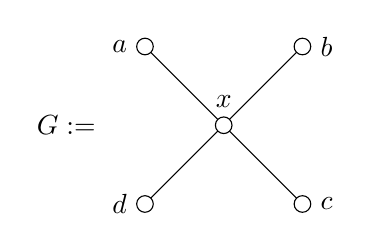
\begin{tikzpicture}
        \tikzset{
          dot/.style = {circle, draw, fill=white, minimum size=#1, inner sep=0pt, outer sep=0pt},
          dot/.default = 6pt
        }
        \node[label=center:{\(G :=\)}] (G) at (-1,1) {};
        \node[dot,label=left:{\(a\)}] (a) at (0,2) {};
        \node[dot,label=right:{\(b\)}] (b) at (2,2) {};
        \node[dot,label=right:{\(c\)}] (c) at (2,0) {};
        \node[dot,label=left:{\(d\)}] (d) at (0,0) {};
        \node[dot,label=above:{\(x\)}] (x) at (1,1) {};

        \draw (a) -- (x);
        \draw (b) -- (x);
        \draw (c) -- (x);
        \draw (d) -- (x);
      \end{tikzpicture}
      \end{center}

      In this graph \(k(G) = 1\), and setting \(V' = \{x\}\) yields \(\omega(G - V') = 4\).
  \end{enumerate} \n



  \itm{3.1.2} Show that if \(G\) is \(k\)-edge-connected, then \(\varepsilon \geq \displaystyle\frac{k \nu}{2}\). \n
    \begin{align*}
      \varepsilon &= \frac12 \left(\sum_{v \in V} d_G(v)\right) & (\text{theorem 1.1}) \\
                  &\geq \frac12 \left(\sum_{v \in V} \delta \right) & \left(\delta = \min \{d_G(v) \mid v \in V\}\right) \\
                  &= \frac{\delta \nu}{2} & (\nu = |V|) \\
                  &\geq \frac{k \nu}{2} & (\text{theorem 3.1}).
    \end{align*} \n
  



  \itm{3.2.2} Give an example to show that if \(P\) is a \((u,v)\)-path in a 2-connected graph \(G\), then \(G\) does not necessarily contain a \((u,v)\)-path \(Q\) internally-disjoint from \(P\).

      \begin{center}
      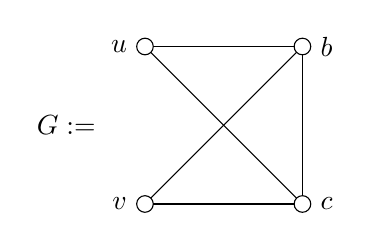
\begin{tikzpicture}
        \tikzset{
          dot/.style = {circle, draw, fill=white, minimum size=#1, inner sep=0pt, outer sep=0pt},
          dot/.default = 6pt
        }
        \node[label=center:{\(G :=\)}] (G) at (-1,1) {};
        \node[dot,label=left:{\(u\)}] (a) at (0,2) {};
        \node[dot,label=right:{\(b\)}] (b) at (2,2) {};
        \node[dot,label=right:{\(c\)}] (c) at (2,0) {};
        \node[dot,label=left:{\(v\)}] (d) at (0,0) {};

        \draw (a) -- (b) -- (c) -- (d);
        \draw (b) -- (d);
        \draw (a) -- (c);
      \end{tikzpicture}
      \end{center}
      This graph is clearly 2-connected.  Now take path \(P = ubcv\), since \(uv\) isn't a path, there exists no path \(Q\) that doesn't contain vertices \(b\) or \(c\).  So \(P\) and \(Q\) cannot be internally-disjoint. \n

      This doesn't contradict theorem 3.2 though.  For example, take \(P = ubv\), there's still internally-disjoint path \(Q = ucv\).

\end{itemize}
\end{document}
